\documentclass[9pt,aspectratio=169,xcolor=table]{beamer}

%~~~~~~~~~~~~~~~~~~~~~~~~~~~~~~~~~~~~~~~~~~~~~~~~~~~~~~~~~~~~~~~~~~~~~~~~~~~~~~
% Use roboto Font (recommended)
\usepackage[sfdefault]{roboto}
\usepackage[utf8]{inputenc}
\usepackage[T1]{fontenc}
%~~~~~~~~~~~~~~~~~~~~~~~~~~~~~~~~~~~~~~~~~~~~~~~~~~~~~~~~~~~~~~~~~~~~~~~~~~~~~~

%~~~~~~~~~~~~~~~~~~~~~~~~~~~~~~~~~~~~~~~~~~~~~~~~~~~~~~~~~~~~~~~~~~~~~~~~~~~~~~
% Define where theme files are located. ('/styles')
\usepackage{styles/fluxmacros}
\usefolder{styles}
% Use Flux theme v0.1 beta
% Available style: asphalt, blue, red, green, gray
\usetheme[style=gray]{flux}
%~~~~~~~~~~~~~~~~~~~~~~~~~~~~~~~~~~~~~~~~~~~~~~~~~~~~~~~~~~~~~~~~~~~~~~~~~~~~~~

%~~~~~~~~~~~~~~~~~~~~~~~~~~~~~~~~~~~~~~~~~~~~~~~~~~~~~~~~~~~~~~~~~~~~~~~~~~~~~~
% Extra packages
\usepackage{booktabs}
\usepackage{colortbl}
\usepackage{ragged2e}
\usepackage{amssymb}
\usepackage{multirow}
\usepackage{tikz}
\usetikzlibrary{arrows.meta, positioning, fit, backgrounds, calc, decorations.pathreplacing}
\setbeamertemplate{itemize items}[square]
\usepackage[scaled=.92]{beramono}
\usepackage{listings}
\usepackage{styles/lstlangarm}
\usepackage{array}
\definecolor{bgcolor}{HTML}{F2E9E9}
% lstlangarm.sty references \color{mauve} for string literals but never defines
% it -- only fires when a listing contains a string. Define it here.
\definecolor{mauve}{rgb}{0.58,0,0.82}
% lstlangarm's C style sets commentstyle=green!20, which is unreadable on the
% pink listing background. Darken it globally.
\lstset{commentstyle=\color{green!45!black}}
% ragged-right fixed-width column -- must be defined in the preamble, never
% inside a frame (\newcolumntype's #1 breaks beamer's frame scanner)
\newcolumntype{R}[1]{>{\RaggedRight\arraybackslash}p{#1}}
%~~~~~~~~~~~~~~~~~~~~~~~~~~~~~~~~~~~~~~~~~~~~~~~~~~~~~~~~~~~~~~~~~~~~~~~~~~~~~~
% Table striping: odd rows white, even rows very light gray.
% Needs \documentclass[...,xcolor=table]{beamer} (beamer loads xcolor itself,
% so the option must go on the class, not \usepackage).
\definecolor{stripe}{gray}{0.94}
% \striped makes body rows alternate white, gray, white, ... starting white.
% \rowcolors counts from the first coloured body row; the header is not counted.
\newcommand{\striped}{\rowcolors{1}{white}{stripe}}
%~~~~~~~~~~~~~~~~~~~~~~~~~~~~~~~~~~~~~~~~~~~~~~~~~~~~~~~~~~~~~~~~~~~~~~~~~~~~~~

%~~~~~~~~~~~~~~~~~~~~~~~~~~~~~~~~~~~~~~~~~~~~~~~~~~~~~~~~~~~~~~~~~~~~~~~~~~~~~~
% TikZ block styles -- matches ch1/ch2
% Colour variables are named identically in the book's stm32primer.tex, so any
% tikzpicture using only the \tikzset{...} styles below can be copied verbatim
% between slides and book. Only the \definecolor/\colorlet VALUES differ: the
% book is printed, so it keeps every stroke pure black with muted fills. These
% slides are projected, so both fill AND stroke are bright and saturated to
% grab attention -- see stm32primer.tex for the print palette.
\definecolor{blkfill}{HTML}{DCEBFF}
\definecolor{blkline}{HTML}{1565C0}
\definecolor{accentfill}{HTML}{FFE0B2}
\definecolor{accentline}{HTML}{E65100}
\definecolor{memfill}{HTML}{DFF5DA}
\definecolor{memline}{HTML}{2E7D32}
\definecolor{cellfill}{HTML}{FFFFFF}
\definecolor{cellline}{HTML}{424242}
\definecolor{bitmaskfill}{HTML}{DCEBFF}
\definecolor{bitmaskline}{HTML}{1565C0}
\definecolor{bithitfill}{HTML}{FFE0B2}
\definecolor{bithitline}{HTML}{E65100}
\tikzset{
  blk/.style   = {rectangle, rounded corners=2pt, draw=blkline, fill=blkfill,
                  thick, align=center, font=\small, minimum height=9mm, inner sep=3pt},
  cpublk/.style= {rectangle, rounded corners=2pt, draw=accentline, fill=accentfill,
                  thick, align=center, font=\small\bfseries, minimum height=9mm, inner sep=3pt},
  memblk/.style= {rectangle, rounded corners=2pt, draw=memline, fill=memfill,
                  thick, align=center, font=\small, minimum height=9mm, inner sep=3pt},
  cell/.style  = {rectangle, draw=cellline, fill=cellfill, align=center,
                  font=\normalsize\ttfamily, minimum height=7mm, inner sep=2pt},
  lbl/.style   = {font=\scriptsize, text=Gray},
  flow/.style  = {-{Stealth[length=2mm]}, thick, draw=blkline},
  busline/.style={thick, draw=cellline},
}
% NOTE (theme quirks -- all fail SILENTLY, always page through the PDF):
%  - a second \\ inside a nested {...} group in a TikZ node breaks parsing
%  - {\small ...} wrapped around a nested itemize eats the frame title + list
%  - \usebeamercolor on a [plain] frame falls through to an unstyled default
%  - \newcolumntype inside a frame breaks beamer's frame scanner
%  - lstlisting needs \begin{frame}[fragile]
%  - a TikZ picture wider than its column silently overflows into neighbours
%~~~~~~~~~~~~~~~~~~~~~~~~~~~~~~~~~~~~~~~~~~~~~~~~~~~~~~~~~~~~~~~~~~~~~~~~~~~~~~

%%%%%%%%%%%%%%%%%%%%%%%%%%%%%%%%%%%
%% BEGIN CONDITIONAL COMPILATION %%
%%%%%%%%%%%%%%%%%%%%%%%%%%%%%%%%%%%
\newif\ifwebex
%\webextrue % uncomment to generate section separator
\ifwebex
\AtBeginSection[]{
  \begin{frame}
  \vfill
  \centering
  \begin{beamercolorbox}[sep=8pt,center,shadow=true,rounded=true]{title}
    \usebeamerfont{title}\insertsectionhead\par%
  \end{beamercolorbox}
  \vfill
  \end{frame}
}
\else
\AtBeginSection[]
{
{
    \setbeamercolor{background canvas}{bg=yellow!10}
    \begin{frame}[plain]
        \frametitle{Table of Contents}
        \tableofcontents[currentsection]
    \end{frame}
}
}
\fi
%%%%%%%%%%%%%%%%%%%%%%%%%%%%%%%%%%%
%% END CONDITIONAL COMPILATION   %%
%%%%%%%%%%%%%%%%%%%%%%%%%%%%%%%%%%%

%~~~~~~~~~~~~~~~~~~~~~~~~~~~~~~~~~~~~~~~~~~~~~~~~~~~~~~~~~~~~~~~~~~~~~~~~~~~~~~
% Information
\title{General Purpose Input Output}
\subtitle{\emph{Introduction to ARM Cortex-M Microprocessors} --- Chapter 8}
\author{Mun\'{i}m Zabidi}
\institute{\color{primary}Faculty of Electrical Engineering, Universiti Teknologi Malaysia}
\date{\today}
\titlegraphic{assets/logoutmwhite.png}
%~~~~~~~~~~~~~~~~~~~~~~~~~~~~~~~~~~~~~~~~~~~~~~~~~~~~~~~~~~~~~~~~~~~~~~~~~~~~~~

\begin{document}

\titlepage

\begin{frame}{Table of Contents}
    \tableofcontents
\end{frame}

%===============================================================================
\section{Why This Matters}
%===============================================================================

\begin{frame}{Why This Chapter Matters}
    \leavevmode
    Chapter~4 already blinked an LED in C. Chapters~5--7 then opened up what that program became underneath --- the load, the mask, the store, the branch. This chapter closes the loop: the same \texttt{MODER}/\texttt{ODR} pattern you have now seen at both levels becomes the foundation for every peripheral in the rest of this book. A GPIO pin is the simplest bridge between software and the physical world, so it is where that pattern is easiest to see start to finish.
\end{frame}

\begin{frame}{Objectives}
    \leavevmode
    {\small After completing this chapter, you should be able to:}

    \vspace{2mm}
    {\small
    \begin{enumerate}\itemsep2pt
        \item Describe the parts inside a GPIO pin: the Schmitt trigger, the output driver, and the pull resistors.
        \item Choose between push-pull and open-drain outputs for a given external circuit.
        \item Configure any pin's mode, output type, speed, and pull resistors using the GPIO registers.
        \item Explain why a peripheral clock must be enabled before its registers respond.
        \item Use \texttt{BSRR} for atomic pin changes, and explain why it beats a read-modify-write on \texttt{ODR}.
        \item Read a switch input reliably, including software debouncing.
        \item Drive a multi-segment display from a lookup table instead of per-segment logic.
    \end{enumerate}}
\end{frame}


%===============================================================================
\section{Inside a GPIO Pin}
%===============================================================================

\begin{frame}[plain]{Inside a GPIO Pin}
    \begin{center}
    \includegraphics[width=.86\textwidth, height=.66\textheight, keepaspectratio]%
        {assets/gpio-pin.pdf}
    \end{center}

    \vspace{1mm}
    {\small\centering One pin has two separate paths: an \alert{input} path
    through a Schmitt trigger to \texttt{IDR}, and an \alert{output} path from
    \texttt{ODR} through the driver transistors. Pull resistors sit in between.\par}
\end{frame}

\begin{frame}{Push-Pull and Open-Drain}
    \begin{columns}[c]
    \begin{column}{.48\textwidth}
        \begin{center}
        \includegraphics[width=\textwidth, height=.42\textheight, keepaspectratio]%
            {assets/pushpull.pdf}
        \end{center}
        {\scriptsize\centering \textbf{Push-pull} --- drives both high and low\par}
    \end{column}
    \begin{column}{.48\textwidth}
        \begin{center}
        \includegraphics[width=\textwidth, height=.42\textheight, keepaspectratio]%
            {assets/opendrain.pdf}
        \end{center}
        {\scriptsize\centering \textbf{Open-drain} --- pulls low, or releases\par}
    \end{column}
    \end{columns}

    \vspace{2mm}
    \begin{block}{When you need open-drain}
        Push-pull is the default. It is what you want for an LED. But if
        two devices share one wire, one driving high while the other
        drives low causes a \alert{short circuit}. Open-drain lets many
        devices share one line safely. This is exactly how
        I\textsuperscript{2}C works (Chapter 13).
    \end{block}
\end{frame}

\begin{frame}{Pull-Up and Pull-Down}
    \begin{columns}[c]
    \begin{column}{.5\textwidth}
        \begin{center}
        \includegraphics[width=\textwidth, height=.36\textheight, keepaspectratio]%
            {assets/pullup-circuit.pdf}
        \end{center}
    \end{column}
    \begin{column}{.5\textwidth}
        \begin{center}
        \includegraphics[width=\textwidth, height=.36\textheight, keepaspectratio]%
            {assets/pulldown-circuit.pdf}
        \end{center}
    \end{column}
    \end{columns}

    \vspace{2mm}
    \begin{block}{An unconnected input \emph{floats}}
        It picks up noise and reads a random value. A pull resistor gives
        it a fixed level when nothing else is driving it.

        \vspace{1mm}
        A button wired to ground needs a \alert{pull-up}, so
        \alert{pressed reads 0}. This is called active-low.
        \texttt{PUPDR} can turn on a pull-up inside the chip, so you do
        not need an extra part.
    \end{block}
\end{frame}

\begin{frame}[plain]{\texttt{PUPDR} --- The Internal Resistors}
    \begin{center}
    \includegraphics[width=.92\textwidth, height=.56\textheight, keepaspectratio]%
        {assets/pupdr-modes.pdf}
    \end{center}

    \vspace{1mm}
    {\small\centering Two bits per pin: \texttt{00} floating, \texttt{01}
    pull-up, \texttt{10} pull-down. An internal resistor means
    \alert{one fewer part} on the board. This is Chapter 1's cost
    argument again.\par}
\end{frame}

%===============================================================================
\section{The GPIO Registers}
%===============================================================================

\begin{frame}{The Register Set}
    \begin{center}
    {\small
    \striped
    \begin{tabular}{@{}l l R{.50\textwidth}@{}}
        \toprule
        \textbf{Register} & \textbf{Bits/pin} & \textbf{Purpose} \\
        \midrule
        \texttt{MODER}   & 2 & Mode: input, output, alternate function, analog \\
        \texttt{OTYPER}  & 1 & Output type: push-pull or open-drain \\
        \texttt{OSPEEDR} & 2 & Output slew rate \\
        \texttt{PUPDR}   & 2 & Pull-up, pull-down, or neither \\
        \texttt{IDR}     & 1 & \alert{Input} data --- read the pin \\
        \texttt{ODR}     & 1 & \alert{Output} data --- drive the pin \\
        \texttt{BSRR}    & 2 & Atomic bit set / reset \\
        \texttt{AFR[2]}  & 4 & Which alternate function (Chapter 10) \\
        \bottomrule
    \end{tabular}}
    \end{center}

    \vspace{2mm}
    \begin{block}{Bits per pin tells you how to build the mask}
        One bit wide: mask \texttt{1}, at position $n$.
        Two bits wide: mask \texttt{3}, at position $2n$.
        Four bits wide: mask \texttt{0xF}, at position $4n$.
    \end{block}
\end{frame}

\begin{frame}[plain]{\texttt{MODER} --- Selecting the Mode}
    \begin{center}
    \includegraphics[width=.9\textwidth, height=.42\textheight, keepaspectratio]%
        {assets/moder-bits.pdf}
    \end{center}

    \vspace{2mm}
    \begin{columns}[T]
    \begin{column}{.4\textwidth}
        {\small
        \striped
        \begin{tabular}{@{}l l@{}}
            \toprule
            \textbf{Bits} & \textbf{Mode} \\
            \midrule
            \texttt{00} & Input (reset state) \\
            \texttt{01} & \alert{General-purpose output} \\
            \texttt{10} & Alternate function \\
            \texttt{11} & Analog \\
            \bottomrule
        \end{tabular}}
    \end{column}
    \begin{column}{.56\textwidth}
        {\ttfamily\footnotesize
        GPIOA->MODER \&= \textasciitilde(3U << (5*2));~~// clear \\
        GPIOA->MODER |=~~(1U << (5*2));~~// set 01}

        \vspace{2mm}
        {\small \alert{Clear first, then set.} Without the clear step, you
        cannot change a \texttt{11} into a \texttt{01}.}
    \end{column}
    \end{columns}
\end{frame}

\begin{frame}[plain]{\texttt{BSRR} --- Atomic Set and Reset}
    \begin{center}
    \includegraphics[width=.9\textwidth, height=.38\textheight, keepaspectratio]%
        {assets/bsrr-bits.pdf}
    \end{center}

    \vspace{2mm}
    \begin{columns}[T]
    \begin{column}{.46\textwidth}
        {\small \texttt{ODR |= x} is a \alert{read-modify-write}: three
        separate steps. If an interrupt changes another pin in between,
        that change is \alert{lost}.}
    \end{column}
    \begin{column}{.5\textwidth}
        {\ttfamily\footnotesize
        GPIOA->BSRR = (1U << 5);~~~~~~// PA5 on \\
        GPIOA->BSRR = (1U << (5+16));~// PA5 off}

        \vspace{2mm}
        {\small One \alert{write}, no read. Note the \texttt{=} instead of
        \texttt{|=}. Using \texttt{|=} here would be a bug.}
    \end{column}
    \end{columns}
\end{frame}

\begin{frame}[plain]{Peripheral Clock Gating}
    \begin{center}
    \includegraphics[width=.9\textwidth, height=.40\textheight, keepaspectratio]%
        {assets/ahb1enr-bits.pdf}
    \end{center}

    \vspace{2mm}
    \begin{block}{The classic first bug}
        Every peripheral starts with its clock \alert{disabled}, to save
        power. A peripheral with no clock \alert{does not respond to
        writes}: the writes are simply lost. No fault, no error, nothing
        happens.

        \vspace{1mm}
        {\ttfamily\normalsize RCC->AHB1ENR |= (1U << 0);~~// GPIOA}
    \end{block}
\end{frame}

%===============================================================================
\section{Experiments}
%===============================================================================

\begin{frame}[fragile]{Experiment 1--2: Blink an LED}
    \begin{columns}[T]
    \begin{column}{.5\textwidth}
        \textbf{With \texttt{ODR}}
\begin{lstlisting}[style=myc, basicstyle=\ttfamily\scriptsize]
#include "stm32f4xx.h"
void delay_ms(uint32_t ms) { for (uint32_t i=0;i<ms*4000;i++) __NOP(); }
int main(void) {
    RCC->AHB1ENR |= (1U << 0);
    GPIOA->MODER &= ~(3U << 10);
    GPIOA->MODER |=  (1U << 10);
    while (1) {
        GPIOA->ODR |=  (1U << 5);
        delay_ms(500);
        GPIOA->ODR &= ~(1U << 5);
        delay_ms(500);
    }
}
\end{lstlisting}
    \end{column}
    \begin{column}{.46\textwidth}
        \textbf{With \texttt{BSRR}}
\begin{lstlisting}[style=myc, basicstyle=\ttfamily\scriptsize]
#include "stm32f4xx.h"
void delay_ms(uint32_t ms) { for (uint32_t i=0;i<ms*4000;i++) __NOP(); }
int main(void) {
    RCC->AHB1ENR |= (1U << 0);
    GPIOA->MODER &= ~(3U << 10);
    GPIOA->MODER |=  (1U << 10);
    while (1) {
        GPIOA->BSRR = (1U << 5);
        delay_ms(500);
        GPIOA->BSRR = (1U << 21);
        delay_ms(500);
    }
}
\end{lstlisting}

        \vspace{2mm}
        {\small Same effect, but the second version is \alert{atomic} and
        one instruction shorter.}
    \end{column}
    \end{columns}

    \vspace{2mm}
    {\small $5 \times 2 = 10$, so \texttt{PA5}'s mode bits sit at position
    10. $5 + 16 = 21$ is its reset bit in \texttt{BSRR}.}
\end{frame}


\begin{frame}[fragile]{Experiment 3: Button Controls LED}
    \begin{columns}[T]
    \begin{column}{.52\textwidth}
\begin{lstlisting}[style=myc, basicstyle=\ttfamily\scriptsize]
#include "stm32f4xx.h"
int main(void) {
    RCC->AHB1ENR |= (1U << 2) | (1U << 0);  // GPIOC, GPIOA
    GPIOA->MODER &= ~(3U << 10);
    GPIOA->MODER |=  (1U << 10);       // PA5 output (LED)
    GPIOC->MODER &= ~(3U << (13*2));   // PC13 input
    GPIOC->PUPDR &= ~(3U << (13*2));
    GPIOC->PUPDR |=  (1U << (13*2));   // pull-up

    while (1) {
        if (!(GPIOC->IDR & (1U << 13))) {
            GPIOA->BSRR = (1U << 5);        // pressed -> on
        } else {
            GPIOA->BSRR = (1U << (5+16));   // released -> off
        }
    }
}
\end{lstlisting}
    \end{column}
    \begin{column}{.44\textwidth}
        \begin{center}
        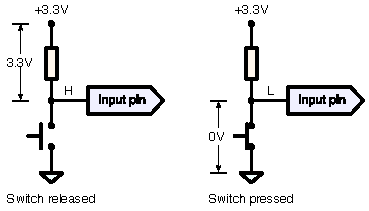
\includegraphics[width=.85\textwidth]{assets/pullup-circuit.pdf}
        \end{center}
    \end{column}
    \end{columns}

    \vspace{2mm}
    {\small The button is \alert{active low}: pressed reads \texttt{0}.
    When released, the $\sim$40~k$\Omega$ pull-up holds the pin HIGH.
    When pressed, the switch gives a low-resistance path to ground.
    That path wins.}
\end{frame}

\begin{frame}{The Other Convention: Pull-Down}
    \begin{center}
    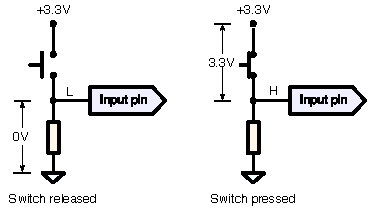
\includegraphics[width=.5\textwidth]{assets/pulldown-circuit.pdf}
    \end{center}

    \vspace{2mm}
    {\small A pull-down with an \alert{active-high} switch is the mirror
    image: released reads LOW, and pressed connects the pin to
    $V_{DD}$. Use \texttt{PUPDR = 10} instead of \texttt{01}, and change
    the polarity in the code to match.}
\end{frame}


\begin{frame}[plain]{Experiment 4: Why a Button Needs Debouncing}
    \begin{center}
    \includegraphics[width=.82\textwidth, height=.56\textheight, keepaspectratio]%
        {assets/keybounce.pdf}
    \end{center}

    \vspace{1mm}
    {\small\centering A mechanical contact does not close cleanly. It
    \alert{bounces} for several milliseconds. A processor that polls at
    MHz speed sees one press as \alert{dozens}.\par}
\end{frame}

\begin{frame}[fragile]{Debouncing}
    \begin{columns}[T]
    \begin{column}{.52\textwidth}
\begin{lstlisting}[style=myc, basicstyle=\ttfamily\scriptsize]
#include "stm32f4xx.h"
void delay_ms(uint32_t ms) { for (uint32_t i=0;i<ms*4000;i++) __NOP(); }
void handle_press(void) { /* app-specific action */ }

int main(void) {
    RCC->AHB1ENR |= (1U << 2);        // GPIOC clock
    GPIOC->MODER &= ~(3U << (13*2));  // PC13 input
    GPIOC->PUPDR &= ~(3U << (13*2));
    GPIOC->PUPDR |=  (1U << (13*2));  // pull-up

    while (1) {
        if ((GPIOC->IDR & (1U << 13)) == 0) {
            delay_ms(20);              // let it settle
            if ((GPIOC->IDR & (1U << 13)) == 0) {
                // a real press
                while ((GPIOC->IDR & (1U << 13)) == 0)
                    ;                  // wait for release
                handle_press();
            }
        }
    }
}
\end{lstlisting}
    \end{column}
    \begin{column}{.44\textwidth}
        \begin{block}{Mind the brackets}
            In C, \texttt{\&} binds \emph{looser} than \texttt{==}. So
            \texttt{IDR \& (1<<13) == 0} is parsed as
            \texttt{IDR \& ((1<<13) == 0)}, which is always zero.

            \vspace{2mm}
            \alert{Always put brackets around the mask.}
        \end{block}
    \end{column}
    \end{columns}

    \vspace{2mm}
    {\small A 20\,ms delay is the usual choice. It is long enough for a
    mechanical switch to settle, and short enough that a user does not
    notice.}
\end{frame}


\begin{frame}[fragile]{Experiment 5: Measuring Reaction Time}
	\begin{lstlisting}[style=myc, basicstyle=\ttfamily\scriptsize]
#include "stm32f4xx.h"
void delay_ms(uint32_t ms) { for (uint32_t i=0;i<ms*4000;i++) __NOP(); }
volatile uint32_t reaction_ms;      // inspect this in the debugger
int main(void) {
	RCC->AHB1ENR |= (1U << 0) | (1U << 2);  // GPIOA, GPIOC
	GPIOA->MODER &= ~(3U << 10);
	GPIOA->MODER |=  (1U << 10);            // PA5 output (LED)
	GPIOC->MODER &= ~(3U << (13*2));        // PC13 input (button)
	GPIOC->PUPDR &= ~(3U << (13*2));
	GPIOC->PUPDR |=  (1U << (13*2));        // pull-up

	while (1) {
		GPIOA->BSRR = (1U << (5+16));   // LED off
		delay_ms(2000);                 // wait before the cue
		GPIOA->BSRR = (1U << 5);        // LED on: react now

		reaction_ms = 0;
		while (GPIOC->IDR & (1U << 13)) {   // until the button goes LOW
			delay_ms(1);
			reaction_ms++;
		}
		GPIOA->BSRR = (1U << (5+16));   // acknowledge
		delay_ms(1000);
	}
}
	\end{lstlisting}

	{\small This measurement is only as accurate as \texttt{delay\_ms},
		a calibrated software loop. Its timing shifts with compiler
		optimization and clock speed. \alert{A hardware counter would make it
			exact.}}
\end{frame}

\begin{frame}[fragile]{Experiment 6: Knight Rider LED Chaser}
\begin{lstlisting}[style=myc, basicstyle=\ttfamily\footnotesize]
#include "stm32f4xx.h"
void delay_ms(uint32_t ms) { for (uint32_t i=0;i<ms*4000;i++) __NOP(); }

int main(void) {
    RCC->AHB1ENR |= (1U << 1);      // enable GPIOB clock
    GPIOB->MODER &= ~(0xFFFFU);     // clear PB0..PB7
    GPIOB->MODER |=  (0x5555U);     // PB0..PB7 as outputs (01 each)

    int pos = 0, dir = 1;
    while (1) {
        GPIOB->BSRR = (0xFFU << 16);   // all eight LEDs off
        GPIOB->BSRR = (1U << pos);     // light only the current one

        if (pos == 7 || pos == 0) dir = -dir;  // bounce at the ends
        pos += dir;

        delay_ms(80);
    }
}
\end{lstlisting}

    \vspace{2mm}
    \begin{block}{One lit bit, walking back and forth}
        Only one output pin is ever high at a time; everything else is
        cleared first with a single \alert{atomic} \texttt{BSRR} write,
        then the new bit is set with a second write. \texttt{pos} does
        the work a hardware shift register would do in an all-analogue
        version of this circuit --- flipping \texttt{dir} at each end
        turns a shift into a \alert{bounce}.
    \end{block}
\end{frame}



\begin{frame}[plain]{Experiment 7: A Seven-Segment Display}
    \begin{columns}[c]
    \begin{column}{.4\textwidth}
        \begin{center}
        \includegraphics[width=\textwidth, height=.45\textheight, keepaspectratio]%
            {assets/sevenseg.png}
        \end{center}
    \end{column}
    \begin{column}{.15\textwidth}
        \begin{center}
        \includegraphics[width=\textwidth, height=.45\textheight, keepaspectratio]%
            {assets/sevenseg-pinout.png}
        \end{center}
    \end{column}
    \begin{column}{.4\textwidth}
        \begin{center}
        \includegraphics[width=\textwidth, keepaspectratio]%
            {assets/sevenseg-hex.png}
        \end{center}
    \end{column}
    \end{columns}

    \vspace{2mm}
    \begin{block}{Use a lookup table, not per-segment logic}
        Deciding which of seven segments to light for each digit is a
        table, not an algorithm. \alert{One array indexed by the digit}
        replaces a whole page of \texttt{if} statements. It is also
        faster and easier to check.
    \end{block}
\end{frame}

\begin{frame}[fragile]{Common-Anode Lookup Table}
    \begin{columns}[T]
    \begin{column}{.56\textwidth}
\begin{lstlisting}[style=myc, basicstyle=\ttfamily\scriptsize]
#include "stm32f4xx.h"
void delay_ms(uint32_t ms) { for (uint32_t i=0;i<ms*4000;i++) __NOP(); }

// common-anode codes, digits 0-9
// bit0=a ... bit6=g, bit7=dp -- 0 lights the segment
static const uint8_t seg7_ca[10] = {
    0xC0, 0xF9, 0xA4, 0xB0, 0x99,
    0x92, 0x82, 0xF8, 0x80, 0x90
};

int main(void) {
    RCC->AHB1ENR |= (1U << 1);   // enable GPIOB clock
    GPIOB->MODER &= ~(0xFFFFU);  // clear PB0..PB7
    GPIOB->MODER |=  (0x5555U);  // PB0..PB7 as outputs

    uint8_t digit = 0;
    while (1) {
        GPIOB->ODR = seg7_ca[digit];  // already active-low
        digit = (digit + 1) % 10;
        delay_ms(1000);
    }
}
\end{lstlisting}
    \end{column}
    \begin{column}{.40\textwidth}
        \begin{block}{Why the values look inverted}
            \alert{Common-anode} means the shared pin is tied to
            \texttt{VDD}; each segment lights when its own pin is
            pulled \alert{LOW}. So the table is the bitwise complement
            of the familiar common-\emph{cathode} codes: \texttt{0} is
            \texttt{0x3F} for a cathode display but \texttt{0xC0} here.

            \vspace{1mm}
            Because the table is already active-low, driving it is a
            single \texttt{ODR} write --- no inversion in the loop.
        \end{block}
    \end{column}
    \end{columns}
\end{frame}

\begin{frame}{Summary}
    \begin{itemize}
        \item A GPIO \textbf{port} has 16 pins. Each register controls
              all of them, so change only the bits for your pin.
        \item \texttt{MODER} selects \textbf{input / output / alternate /
              analog}. It uses 2 bits per pin, so pin $n$ sits at $2n$.
        \item \textbf{Push-pull} can drive both high and low.
              \textbf{Open-drain} can only pull low, which is what lets
              devices share a wire.
        \item \texttt{ODR} drives a pin, \texttt{IDR} reads one, and
              \texttt{BSRR} sets or resets a pin \textbf{atomically}.
        \item A button is usually \textbf{active-low} with a pull-up,
              and needs \textbf{debouncing}, since contacts bounce for
              a few milliseconds.
        \item Always \textbf{enable the port's clock} first, or writes
              go nowhere.
    \end{itemize}

    \vspace{2mm}
    \begin{block}{Next: Chapter 9 --- Interrupts and Event-Driven Programming}
        Polling a button wastes the whole processor. Next, we let the
        hardware tell us instead.
    \end{block}
\end{frame}

%===============================================================================
\section{Design Challenge}
%===============================================================================

\begin{frame}{Design Challenge}{To be worked on paper, before any code}
    \leavevmode
    \begin{block}{The brief}
        A control panel needs eight indicator LEDs, four momentary buttons, and one output driving a 24~V relay coil through an external transistor.
    \end{block}

    \vspace{2mm}
    {\small Produce the complete pin-level design for the STM32F446RE: which port and pins, which \texttt{MODER} setting for each, push-pull or open-drain for each output, and which pull resistors for each input. Justify the relay output's configuration in particular. Then state how many register writes your design needs to initialize the whole panel, and whether any of them can be combined.}
\end{frame}

\begin{frame}[plain]
    \begin{center}
        \vfill
        {\usebeamerfont{title}\color{primary}\Huge Questions?}
        \vfill
        {\small\color{Gray} \emph{Introduction to ARM Cortex-M Microprocessors} --- Chapter 8}
        \vfill
    \end{center}
\end{frame}

\end{document}

